\begin{question}[ID=1.1, subtitle={Integrali indefiniti — serie 1}, tags={integrali, indefiniti}, difficulty=media]
Risolvi i seguenti integrali indefiniti

\begin{center}\begin{minipage}{0.7\linewidth}
\begin{enumerate}
\item $\int (3x^2 - 5x + 2) \ dx$
\item $\int_{0}^{1} \frac{1}{2x+1} \ dx$
\item $\int \frac{\ln^3 x}{x} \ dx$
\item $\int \sqrt{9 - x^2} \ dx$
\item $\int x \cdot \sin(x) \ dx$
\item $\int \tan(x) \ dx$
\item $\int \frac{2x + 3}{x^2 + 4x - 5} \ dx$
\item $\int \frac{1}{x^2 + 4x + 7} \ dx$
\end{enumerate}
\end{minipage}\end{center}
\begin{solution}
\begin{align*}
\begin{split}
a)& \quad x^3 - \frac{5}{2}x^2 + 2x + C \\[6pt]
b)& \quad \frac{1}{2} \ln|2x+1| \Big|_0^1 = \frac{\ln 3}{2} \\[6pt]
c)& \quad \frac{1}{4} \ln^4 x + C \\[6pt]
d)& \quad \frac{x}{2} \sqrt{9 - x^2} + \frac{9}{2} \arcsin\left( \frac{x}{3} \right) + C \\
\end{split}
\quad\quad
\begin{split}
e)& \quad -x\cos x + \sin x + C \\[6pt]
f)& \quad -\ln|\cos x| + C \\[6pt]
g)& \quad \frac{1}{2} \ln|x-1| + \frac{3}{2} \ln|x+5| + C \\[6pt]
h)& \quad \frac{1}{\sqrt{3}} \arctan\left( \frac{x+2}{\sqrt{3}} \right) + C
\end{split}
\end{align*}
\end{solution}
\end{question}


%-----------------------------------------------%

\begin{question}[ID=1.2, subtitle={Integrali indefiniti — serie 2}, tags={integrali, indefiniti}, difficulty=media]
Risolvi i seguenti integrali indefiniti

\begin{center}\begin{minipage}{0.7\linewidth}
\begin{enumerate}
\item $\int (2x^3 - x^2 + 4x -1) \ dx$
\item $\int \frac{2x+1}{x^2+x} \ dx$
\item $\int \frac{1}{x \cdot \ln x} \ dx$
\item $\int \sqrt{16- x^2} \ dx$
\item $\int x \cdot e^{x} \ dx$
\item $\int \frac{dx}{\cos^2(3x)}$
\item $\int \frac{1}{x^2 + 2x + 10} \ dx$
\item $\int \frac{2x+1}{x^2-9} \ dx$
\end{enumerate}
\end{minipage}\end{center}
\begin{solution}
\begin{align*}
\begin{split}
a)& \quad \frac{1}{2}x^4 - \frac{1}{3}x^3 + 2x^2 - x + C \\
b)& \quad \ln|x(x+1)| + C \\
c)& \quad \ln|\ln x| + C \\
d)& \quad \frac{x}{2} \sqrt{16 - x^2} + 8 \arcsin\left(\frac{x}{4}\right) + C
\end{split}
\quad\quad
\begin{split}
e)& \quad e^x(x - 1) + C \\
f)& \quad \frac{1}{3} \tan(3x) + C \\
g)& \quad \frac{1}{3} \arctan\left(\frac{x+1}{3}\right) + C \\
h)& \quad \ln|x^2 - 9| + \frac{1}{6} \ln\left|\frac{x - 3}{x + 3}\right| + C
\end{split}
\end{align*}
\end{solution}
\end{question}



%-----------------------------------------------%


\begin{question}[ID=2.1, subtitle={Primitiva di $f(x)=\ln x^2$ passante per $(1,1)$}, tags={integrali, primitiva}, difficulty=media]
Tra le primitive della funzione $f(x) = \ln x^2$ determina quella il cui grafico passa per il punto $(1,1)$.
\begin{solution}
\[ F(x) = 2x \ln |x| - 2x + 3 \]
\end{solution}
\end{question}

%-----------------------------------------------%

\begin{question}[ID=2.2, subtitle={Primitiva di $f(x)=\ln(x)/x$ passante per $(1,0)$}, tags={integrali, primitiva}, difficulty=media]
Tra le primitive della funzione $f(x) = \dfrac{\ln x}{x}$ determina quella il cui grafico passa per il punto $(1,0)$.
\begin{solution}
\[ F(x) = \frac{1}{2} (\ln x)^2 - \frac{1}{2} \]
\end{solution}
\end{question}

%-----------------------------------------------%

\begin{question}[ID=2.3, subtitle={Primitiva di $f(x)=xe^{x^2}$ passante per $(0,0)$}, tags={integrali, primitiva}, difficulty=media]
Tra le primitive della funzione $f(x) = x \cdot e^{x^2}$ determina quella il cui grafico passa per il punto $(0,0)$.
\begin{solution}
\[ F(x) = \frac{1}{2} e^{x^2} - \frac{1}{2} \]
\end{solution}
\end{question}

%-----------------------------------------------%

\begin{question}[ID=2.4, subtitle={Primitiva di $f(x)=1/(x^2+1)$ passante per $(1,0)$}, tags={integrali, primitiva}, difficulty=media]
Tra le primitive della funzione $f(x) = \dfrac{1}{x^2 + 1}$ determina quella il cui grafico passa per il punto $(1,0)$.
\begin{solution}
\[ F(x) = \arctan(x) - \frac{\pi}{4} \]
\end{solution}
\end{question}

%-----------------------------------------------%

\begin{question}[ID=3.1, subtitle={Valor medio di $\ln x$ su $[1,2]$}, tags={integrali, valor medio}, difficulty=media]
Trova il valor medio $M$ della funzione $f(x) = \ln x$ su $[1, 2]$ e stabilisci per quale ascissa $c$ vale $f(c) = M$.
\begin{solution}
\[ M = \ln 4 - 1, \quad c = e^{\ln 4 - 1} = \frac{4}{e} \]
\end{solution}
\end{question}

%-----------------------------------------------%

\begin{question}[ID=3.2, subtitle={Valor medio di $\sqrt{x}$ su $[1,4]$}, tags={integrali, valor medio}, difficulty=media]
Trova il valor medio $M$ della funzione $f(x) = \sqrt{x}$ su $[1, 4]$ e stabilisci per quale ascissa $c$ vale $f(c) = M$.
\begin{solution}
\[ M = \frac{14}{9}, \quad c = \frac{196}{81} \]
\end{solution}
\end{question}

%-----------------------------------------------%

\begin{question}[ID=3.3, subtitle={Valor medio di $x^2+1$ su $[0,2]$}, tags={integrali, valor medio}, difficulty=media]
Trova il valor medio $M$ della funzione $f(x) = x^2 + 1$ su $[0, 2]$ e stabilisci per quale ascissa $c$ vale $f(c) = M$.
\begin{solution}
\[ M = \frac{7}{3}, \quad c = \sqrt{\frac{4}{3}} = \frac{2}{\sqrt{3}} \]
\end{solution}
\end{question}

%-----------------------------------------------%

\begin{question}[ID=3.4, subtitle={Valor medio di $\cos x$ su $[0,\pi/2]$}, tags={integrali, valor medio}, difficulty=media]
Trova il valor medio $M$ della funzione $f(x) = \cos x$ su $[0, \dfrac{\pi}{2}]$ e stabilisci per quale ascissa $c$ vale $f(c) = M$.
\begin{solution}
\[ M = \frac{2}{\pi}, \quad c = \arccos\!\left(\frac{2}{\pi}\right) \]
\end{solution}
\end{question}

%-----------------------------------------------%

\begin{question}[ID=3.5, subtitle={Valor medio di $1/(x+1)$ su $[1,3]$}, tags={integrali, valor medio}, difficulty=media]
Trova il valor medio $M$ della funzione $f(x) = \dfrac{1}{x + 1}$ su $[1, 3]$ e stabilisci per quale ascissa $c$ vale $f(c) = M$.
\begin{solution}
\[ M = \frac{\ln 2}{2}, \quad c = \frac{2}{\ln 2} - 1 \]
\end{solution}
\end{question}

%-----------------------------------------------%

\begin{question}[ID=4.1, subtitle={Area della versiera di Agnesi nel primo quadrante}, tags={integrali, area, applicazioni}, difficulty=difficile]
La \textit{versiera di Agnesi} è una curva a cui Gaetana Agnesi ha legato il suo nome nel 1748, una curva che peraltro non fu scoperta da lei, ma da Guido Grandi. Analiticamente è il luogo dei punti di intersezione tra due rette che si muovono in relazione a una circonferenza. La funzione è esprimibile come:
\begin{equation*}
    f(x) = \frac{8a^3}{4a^2 + x^2}
\end{equation*}
\begin{enumerate}
    \item Determina l'area delimitata dalla curva nel primo quadrante, l'asse $x$ e la retta verticale di equazione $x=2$.
    \item Calcolane il valore con $a=1$
\end{enumerate}
\begin{solution}
\begin{enumerate}
    \item $A = \int_0^2 \frac{8a^3}{4a^2 + x^2} \, dx = 4a^2 \arctan\!\left(\frac{1}{a}\right)$
    \item Per $a = 1$: $A = 4 \arctan(1) = \pi$
\end{enumerate}
\end{solution}
\end{question}

%-----------------------------------------------%

\begin{question}[ID=4.2, subtitle={Area tra la parabola $y=-x^2+2x$ e la retta $y=-x$}, tags={integrali, area tra curve}, difficulty=media]
\begin{minipage}[t]{0.65\textwidth}
Calcolare l'area compresa tra la parabola $y = -x^2 + 2x$ \\ e la retta $y = -x$
\end{minipage}
\begin{minipage}[t]{0.35\textwidth}
\centering \vspace{-3\baselineskip}
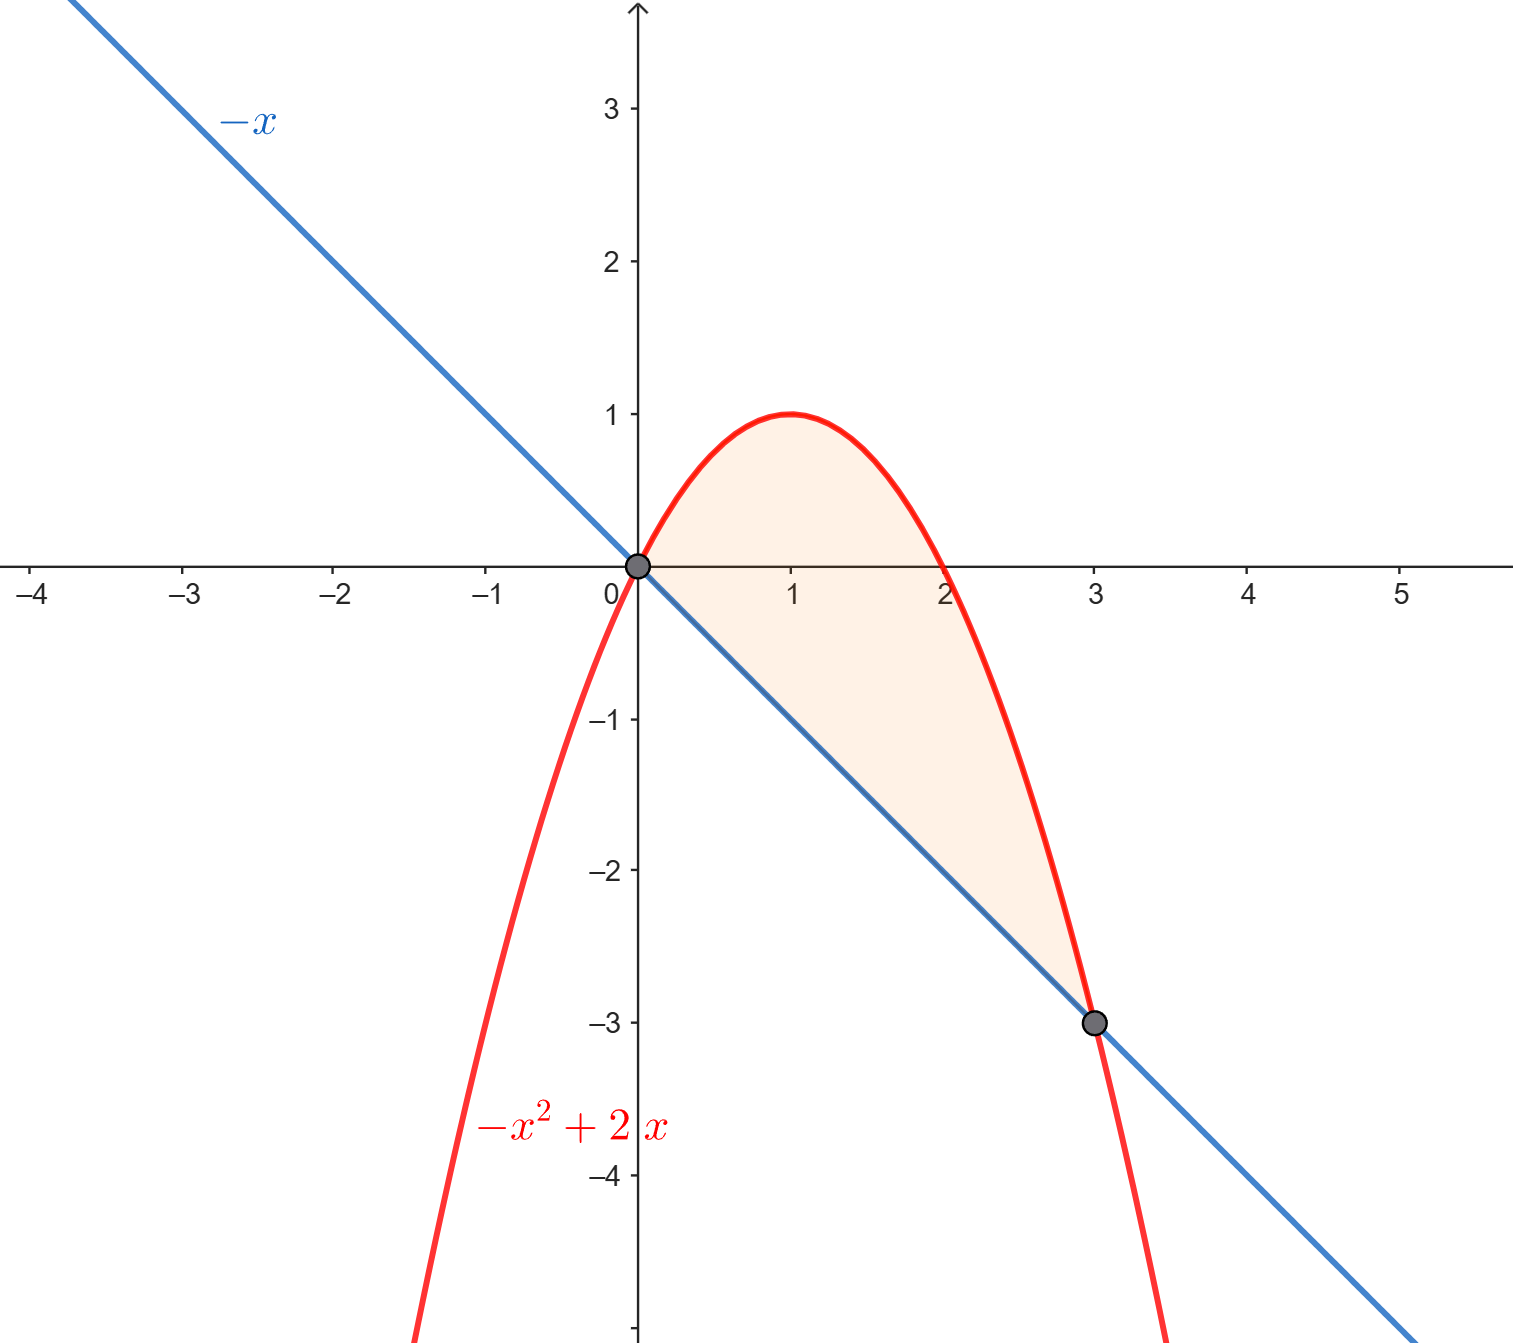
\includegraphics[width=\textwidth]{images/area_tra_curve.png}
\end{minipage}
\begin{solution}
Intersezioni: $-x^2+2x=-x \Rightarrow x(x-3)=0 \Rightarrow x=0,3$.
\[
A = \int_0^3 [(-x^2 + 2x) - (-x)] \, dx = \int_0^3 (-x^2 + 3x) \, dx = \frac{9}{2}
\]
\end{solution}
\end{question}

%-----------------------------------------------%

\begin{question}[ID=5.1, subtitle={Volume della tromba di Torricelli su $[1,2]$}, tags={integrali, volume, solido di rotazione}, difficulty=difficile]
La tromba di Torricelli è un solido ottenuto dalla rivoluzione intorno all'asse $x$ della curva di equazione $y=\dfrac{1}{x}$. Determina il volume del solido di rotazione limitandoti all'intervallo $x \in [1, 2]$
\begin{solution}
\[
V = \pi \int_1^2 \frac{1}{x^2} dx = \pi \left[ -\frac{1}{x} \right]_1^2 = \frac{\pi}{2}
\]
\end{solution}
\end{question}
